\documentclass[final_report.tex]{subfiles}

\begin{document}

\section{Performance Testing \& Evaluation}
\label{sec:evaluation}

This section focusses on the comparison testing which was carried out between the C and Java implementations of basic middleboxes. Evaluation of the results will then be discussed and further improvements to the Java solutions will be considered.

In order to fully understand the capabilities of middleboxes, testing was carried out on Imperial College's Large Scale Distributed Systems (LSDS) test-bed. Although this system consists of numerous machines, tests were carried out using just 2. The first machine was used to host the middlebox application and receive the packets. The other machine was used as the client and ran the pktgen (section \ref{subsec:pktgen}) software allowing it to generate packets at up to 10Gbps in order to take advantage of the machines network interface controllers. Each machine had 2 Intel Xeon ES-2690 2.90Ghz processor which when hyper-threaded, resulted in 32 cores utilising 32GB of memory.

\subsection{Packet Generating}
\label{subsec:pktgen}
Packet generating is the act of creating packets with random payloads to be sent to certain MAC addresses on the network. This can either be done via the use of specialised hardware or using software. They are used for load testing of packet processing applications to test the amount of data which applications can process per second. This can reveal whether limitations on a system is software or hardware based.

\todo[inline]{Talk about pktgen module in kernel - does dpdk version use this}

Pktgen is open source software tool, maintained by Intel, which aims to generate packets using the DPDK framework. It can generate up to 10Gbits of data per second with varying frame sizes ranging from 64 to 1518 bytes, and send the data in the form of packets across a compatible network interface card/controller. It has a number of benefits which include:

\begin{itemize}
	\item Real time packet configuration and port control
	\item Real time metrics on packets sent and received
	\item Handles UDP, TCP, ARP and more packet headers
	\item Can be commanded via a Lua script
\end{itemize}

Pktgen's transmitting performance can be reduced depending on the frame size. This was negated to keep it a constant within the tests by running the application with multiple lcores on the same port with different queues, which allow the transmitting speed to match those of the NIC. With the packet size varying, obviously the number of packets transmitted per second is dependant on this. The differences are shown in Table \ref{tab:pktgen}.

\begin{table}[H]
	\centering
	\begin{tabular} { | c | c | c | }
		\hline
		\textbf{Packet Size} & \textbf{Packet/s (millions)} & \textbf{MBit/s} \\
		\hline
		64 (min) & 14.9 & 9999 \\
		\hline
		128 & 8.4 & 9999 \\
		\hline
		256 & 4.5 & 9999 \\
		\hline
		512 & 2.3 & 9999 \\
		\hline
		1024 & 1.2 & 9999 \\
		\hline
		1518 (max) & 0.8 & 9999 \\
		\hline
	\end{tabular}
	\caption{Pktgen performance for varying packet sizes transmitting in 32 packet burst.}
	\label{tab:pktgen}
\end{table}

\todo{mention constants}

\subsection{C Packet Capture performance test}
The first test on the LSDS test-bed involved comparing the C and Java implementations of a packet capturing application which simply received the packets and freed them straight away without any further transmission. The C implementation is used to give the optimal readings possible from this and further tests, since very limited processing is carried out between receiving and dropping the packet. Figure \ref{fig:pc} shows the performance of the application at varying packet sizes.

\begin{figure}[H]
	\centering
	\begin{subfigure}{0.5\textwidth}
		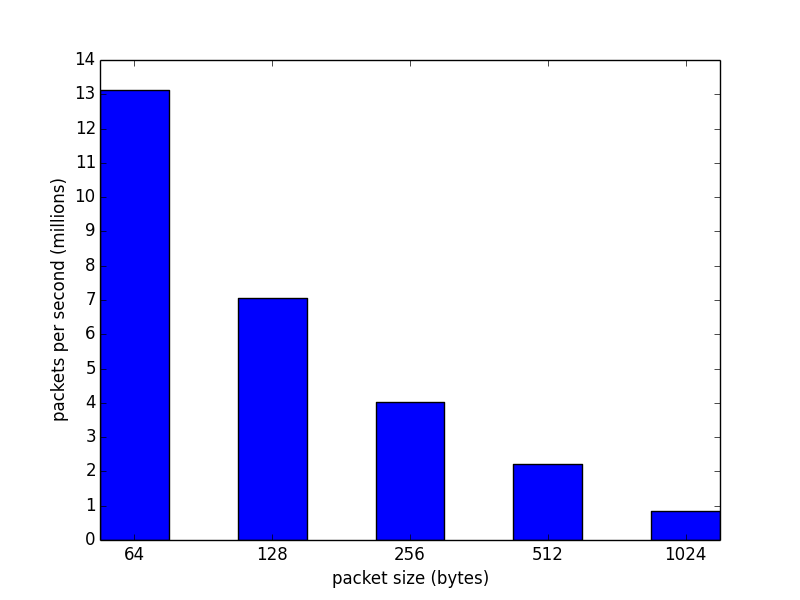
\includegraphics[width=\textwidth]{../../data/pktcap/packets.png}
		\caption{Millions of packets per second}
		\label{fig:pcpackets}
	\end{subfigure}%
	\begin{subfigure}{0.5\textwidth}
		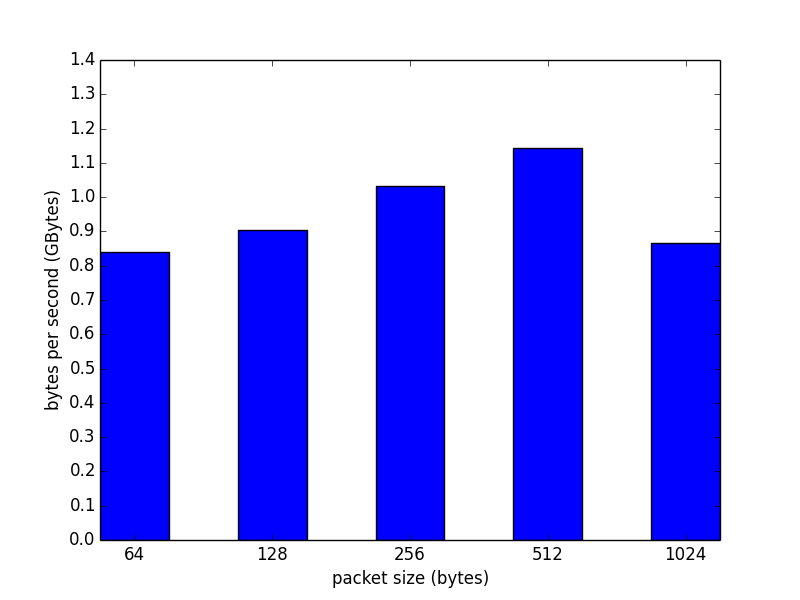
\includegraphics[width=\textwidth]{../../data/pktcap/bytes.png}
		\caption{GBytes per second}
		\label{fig:pcbytes}
	\end{subfigure}
	\caption{Performance results of C implementation of packet capture at varying transmission packet sizes}
	\label{fig:pc}
\end{figure}

Figure \ref{fig:pcpackets} shows the expected results as the packet size increases the number of packets processed per seconds decreases. This is obvious since the NIC has a maximum limit which it can process data per second therefore an inverse correlation between packet size and number of packets exists. If further calculation are carried out, by multiplying the packet size by the number of packets the values turn out to be around the 1000 million bytes per second (1 GBps). This results in roughly 8 Gbps which turns out to be the maximum processing performance of 1 core.

The results of figure \ref{fig:pcbytes} should theoretically have equal bytes per second readings due to the limit of the NIC or the software. However, the results are a lot more skewed than expected and this can be accredited to the memory management of the DPDK framework depending the packet size. Up to a certain limit between 512 bytes and 1024 bytes, DPDK starts splitting packets into multiple segments for storage. This value is determined on a few factors such as the size of the mbuf struct, headroom and pointer sizes.

Although this first test was simple, it showed a few characteristics of fast packet processing. Generally the hardware is more powerful than the software, therefore requiring more than 1 core to handle the received packets of a NIC. Even so, 1 core testing prevails throughout the next tests as to compare with the C results.

\subsection{Java Packet Capture performance test}
The same testing was carried out with an identical packet capture algorithm which was instead implemented in Java using the DPDKJava framework described in section \ref{sec:dpdk}. All testing was done using 64 byte frames to make sure a consistency was kept throughout. Frame size of 64 bytes was chosen as this size is the hardest for applications to process simply because of the sheer number of packets per second which are received. This is an ultimate test of an applications packet throughput, and generally if it can handle packets at 64 bytes, it can handle much larger packets since the packet rate will be reduced. These results are shown in figure \ref{cap}.

\begin{figure}[H]
	\centering
	\begin{subfigure}{0.5\textwidth}
		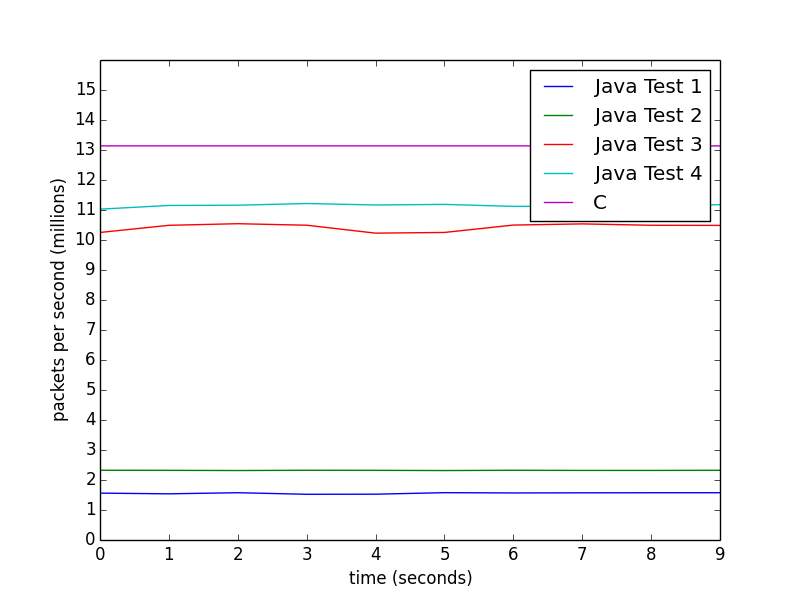
\includegraphics[width=\textwidth]{../../data/pctest1/packets.png}
		\caption{Millions of packets per second}
		\label{fig:cappackets}
	\end{subfigure}%
	\begin{subfigure}{0.5\textwidth}
		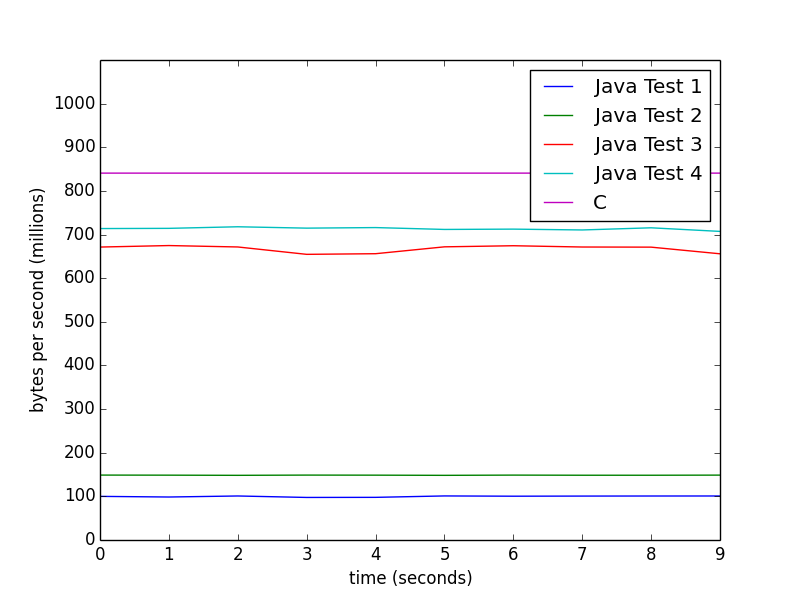
\includegraphics[width=\textwidth]{../../data/pctest1/bytes.png}
		\caption{Millions of bytes per second}
		\label{fig:capbytes}
	\end{subfigure}
	\caption{Performance results of C vs Java implementations of packet capture application for all rounds of testing}
	\label{fig:cap}
\end{figure}

\todo{different frame sizes?}

Figures \ref{fig:cappackets} and \ref{fig:capbytes} indicate that after the first testing using the initial DPDKJava framework that the packet and data throughput was extremely low compared to the C version. Obviously these results are extremely closely related to each other resulting in the C version been roughly 8 times quicker after the first test. Although the native implementation was expected to be slightly quicker, this gap was way too high considering the design considerations and framework implementation.

To check where the problems lied within the code, a Java profiler (JProfiler) was used to check multiple parts of the code including memory usage, CPU usage and the number of method calls and the average time per method call. This provided invaluable analysis of where the problems were, although the profiler significantly reduced the performance of the application since it connects to the JVM and reads the data itself. Even so, obvious bottlenecks could be spotted allowing for performance improvement implementations to be made.

\begin{figure}[H]
	\centering
	\begin{subfigure}{0.5\textwidth}
		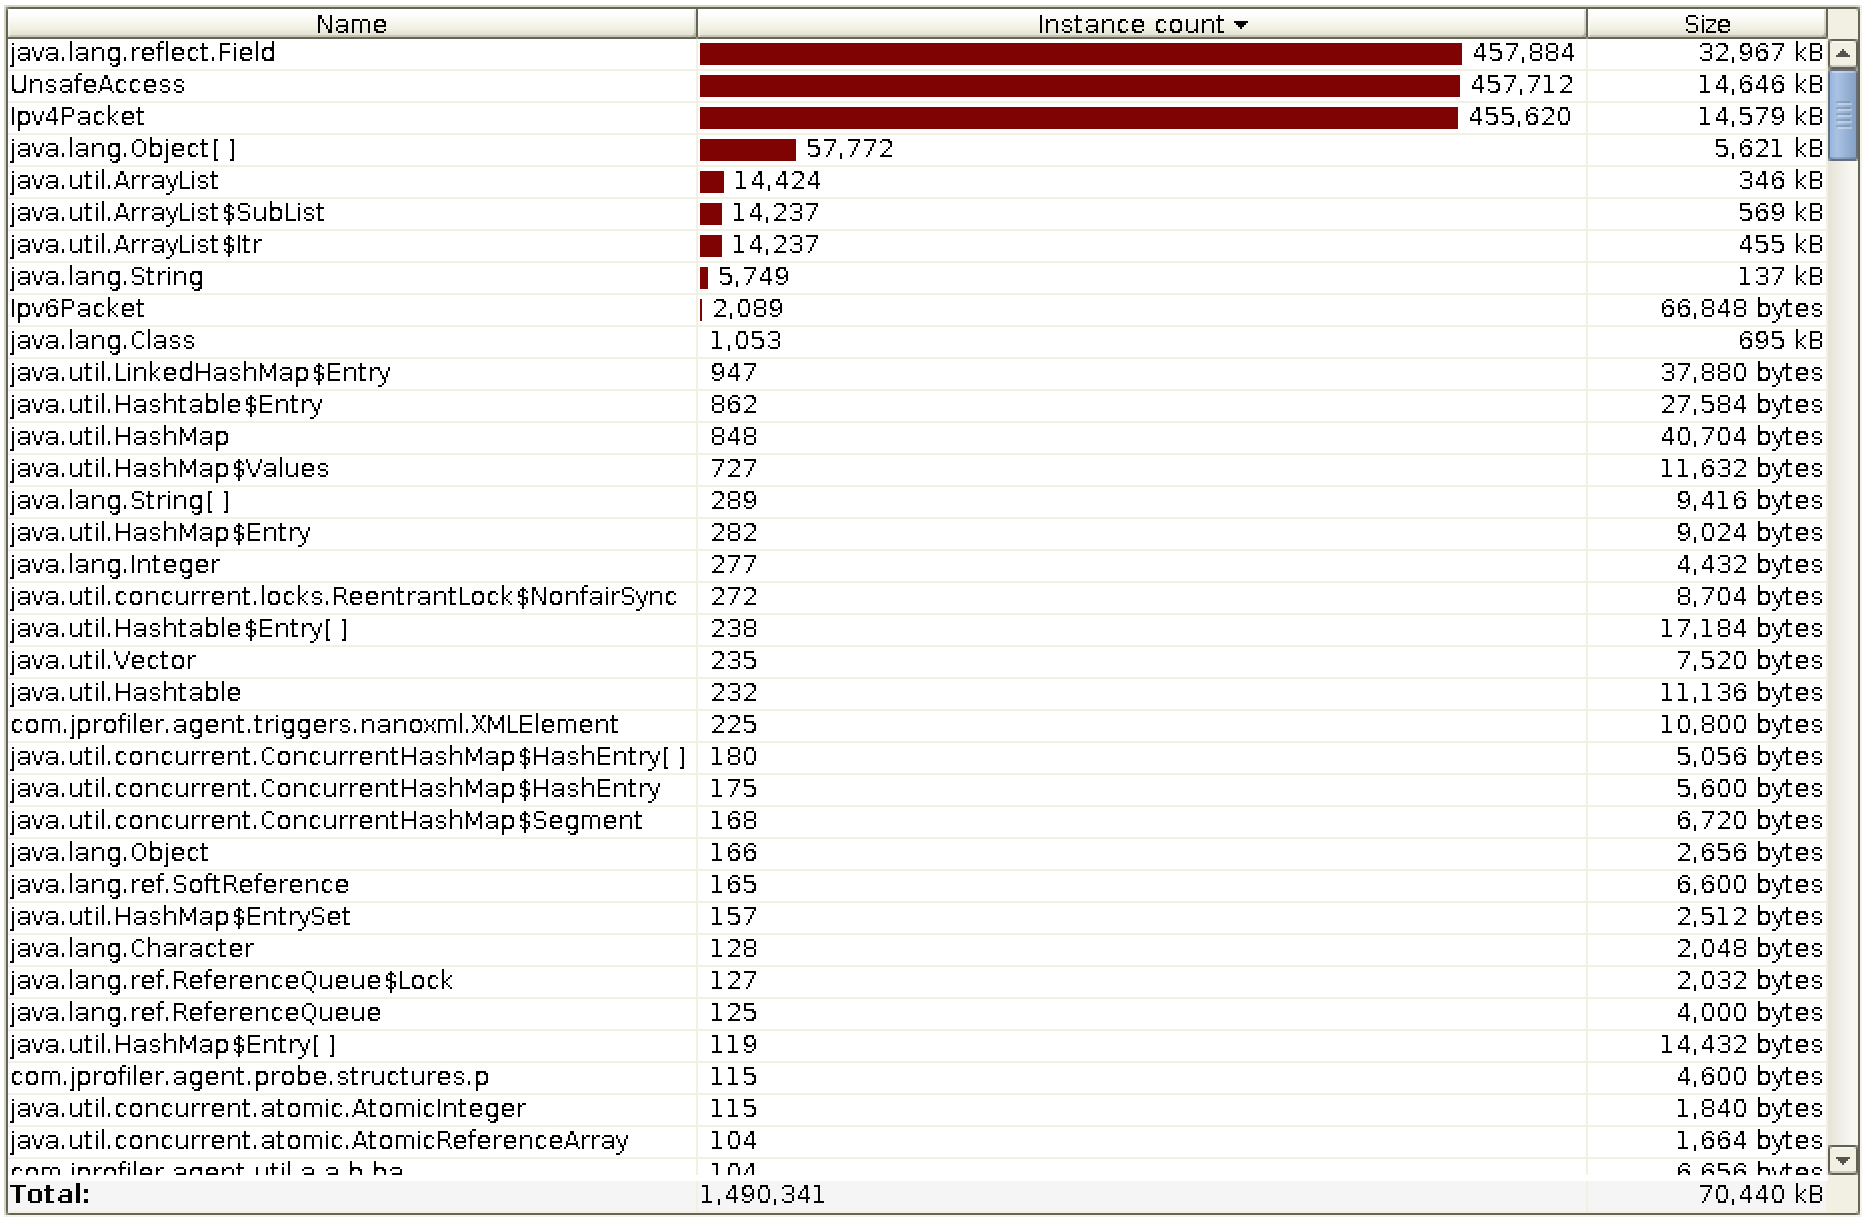
\includegraphics[width=\textwidth]{../../data/pctest1/memory_all_objects.png}
		\caption{Object allocation in memory}
		\label{fig:mem1}
	\end{subfigure}%
	\begin{subfigure}{0.5\textwidth}
		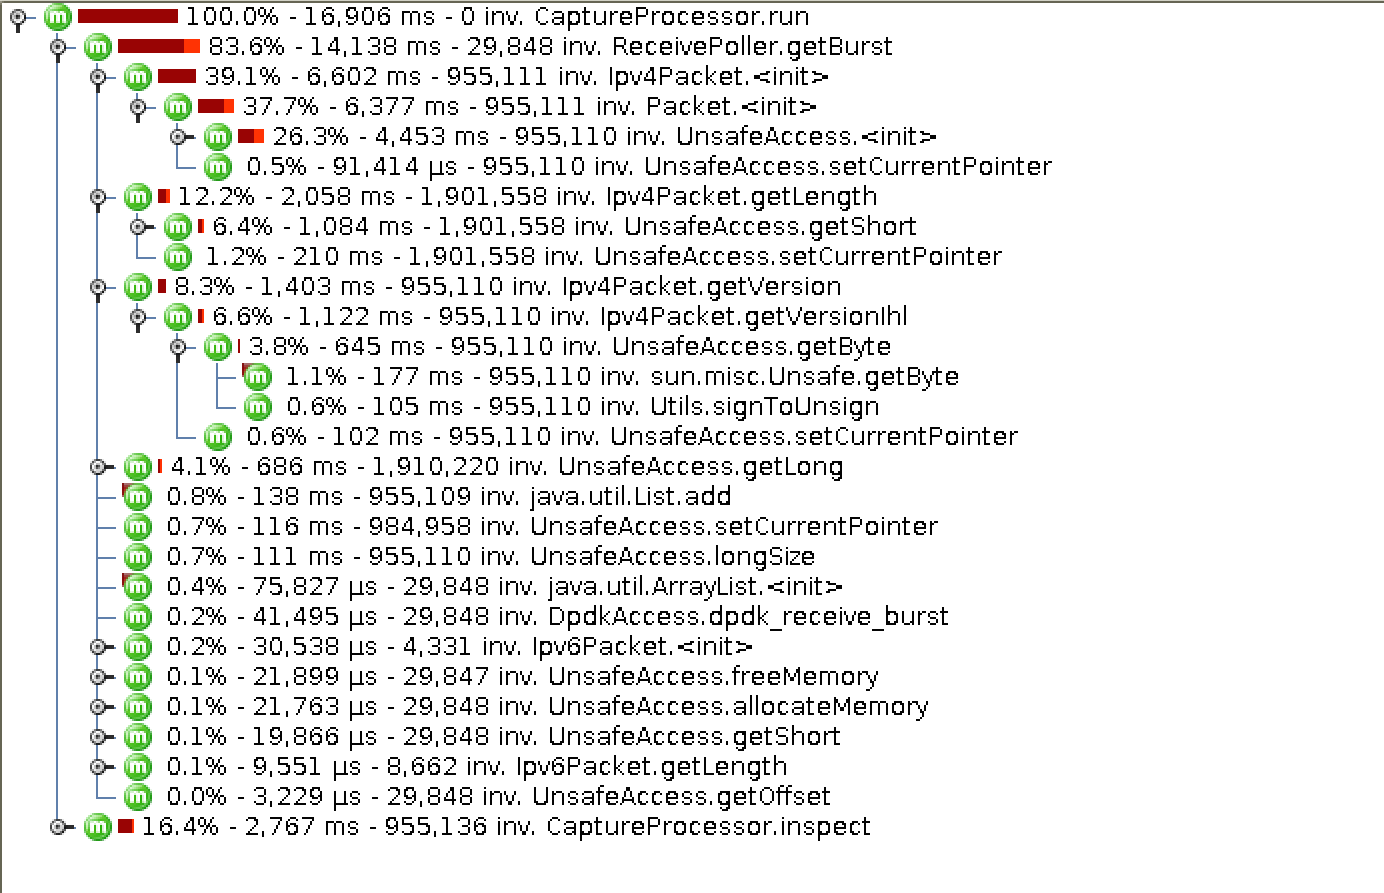
\includegraphics[width=\textwidth]{../../data/pctest1/cpu_call_tree.png}
		\caption{Call tree of most cpu intensive methods}
		\label{fig:cpu1}
	\end{subfigure}
	\caption{Profiler output when analysing the first test of packet capture}
	\label{fig:pro1}
\end{figure}

Figure \ref{fig:pro1} shows some of the output from the profiler which indicated where the main problems were in terms of memory usage and performance. From this, a number of performance upgrades were implemented:

\paragraph*{Capture Processor fields}
The first improvement were to the Packet Capture application itself. The associated processor originally stored the ReceivePoller and PacketFreeer objects within a list to allow for easy iteration if there were numerous objects. Since the Packet Capture application only used 1 of each, separate fields could be used for the objects which removed the list accessing times and iterations.

\paragraph*{Object lifespan}
The other improvements were made to the actual DPDKJava framework. These involved utilising objects throughout the application lifespan instead of creating new ones on every loop. This dramatically reduced the number of initializing methods invoked for the objects and reduced the memory usage in the heap, which reduced the number of times the Java garbage collector was invoked. The class which caused the most problem with this was the ArrayList, which were created on every loop to pass packets through the Java system. Since the framework uses threads without the need to synchronise objects, an ArrayList could be created on initialisation and simply cleared before been used again.

\paragraph*{Off heap allocation}
Finally, instead of allocating new off heap memory to receive the packet pointers through on every loop, a memory bank was allocated on initialisation and the same memory was simply overwritten on every loop iteration. This stopped expensive calls to the allocate and free methods.

Again, the same tests were carried out to check the performance increase of the new framework implementation. Shown in figure \ref{fig:cap} by comparing the blue and green lines, there was a slight performance increase of roughly 1 millions packets per second just by these simple changes, although it was still significantly down on performance to the C version.

Further profiling of the application was undertaken on the improved application. Figure \ref{fig:pro2} shows the analysis which outlined 2 further major improvements which could be made. Each one of these improvements were undertaken and performance tested individual.

\begin{figure}[H]
	\centering
	\begin{subfigure}{0.5\textwidth}
		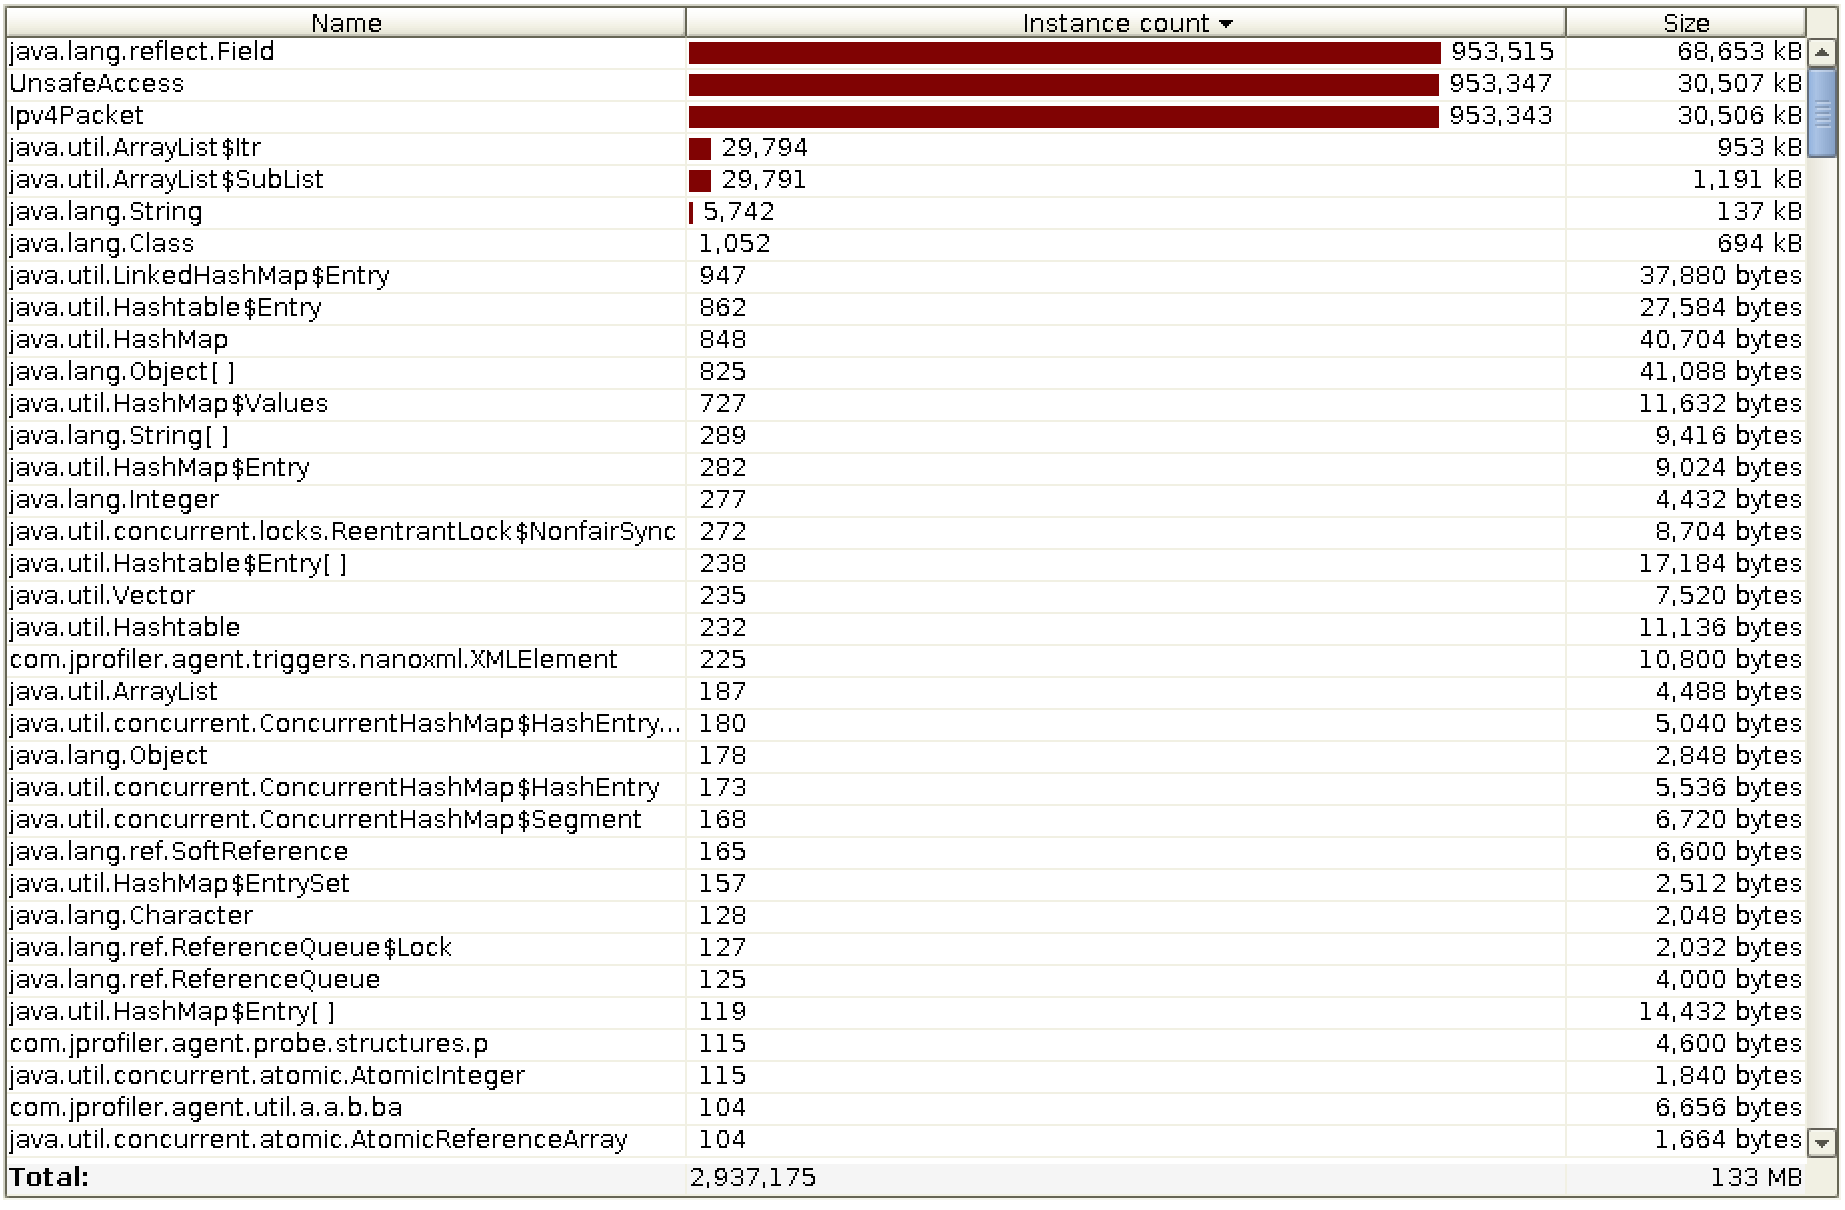
\includegraphics[width=\textwidth]{../../data/pctest2/memory_all_objects.png}
		\caption{Object allocation in memory}
		\label{fig:mem2}
	\end{subfigure}%
	\begin{subfigure}{0.5\textwidth}
		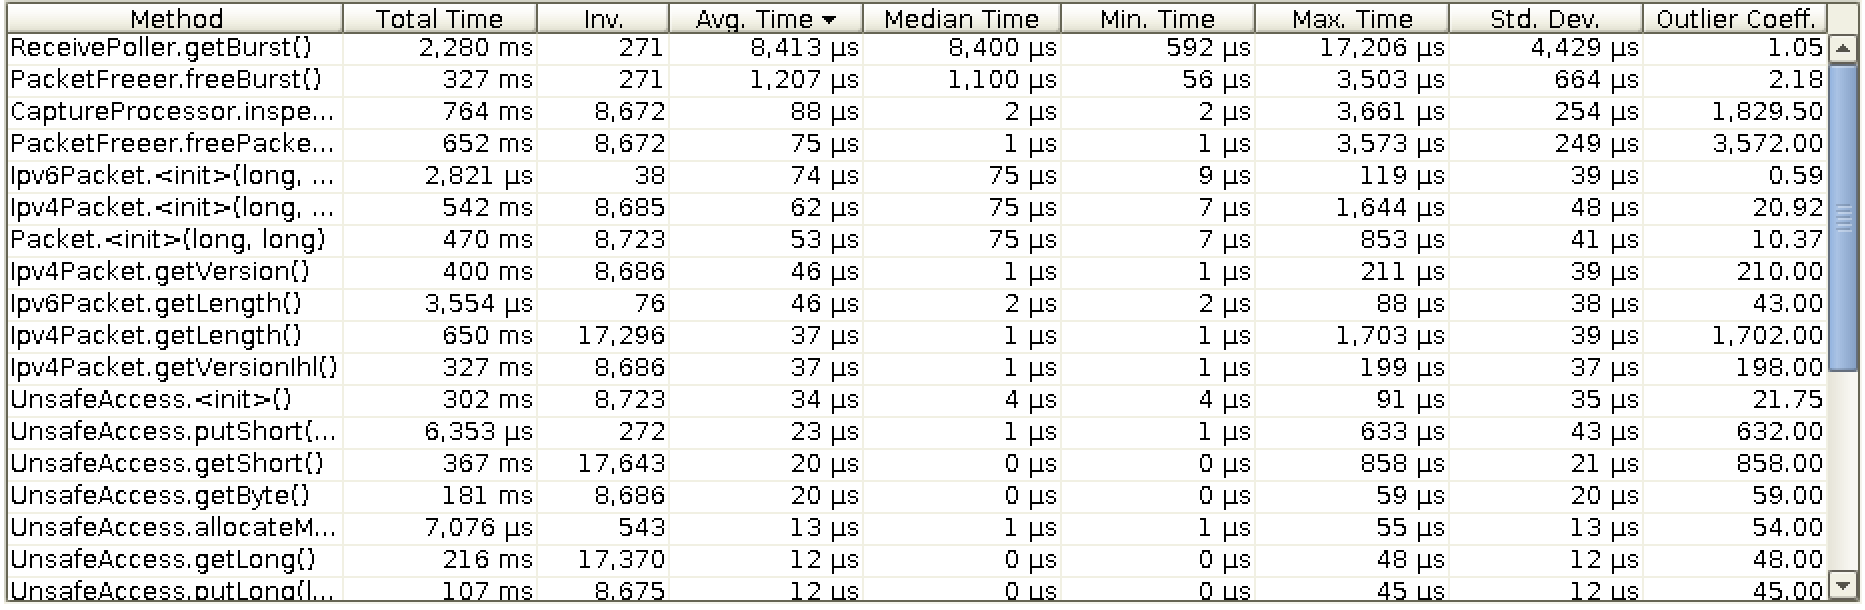
\includegraphics[width=\textwidth]{../../data/pctest1/cpu_methods.png}
		\caption{Most cpu intensive methods along with relevant stats}
		\label{fig:cpu2}
	\end{subfigure}
	\caption{Profiler output when analysing the first test of packet capture}
	\label{fig:pro2}
\end{figure}

\paragraph*{Packet creation}
Of course, for every packet entering the application a packet object is created for easy referencing further down the application pipe-line. However, not using packet objects would significantly reduce the usability and scalability of applications. It was decided not to alter this. However, for each packet initialization a new UnsafeAccess object was been created for use with accessing packet header information. However, since each thread controls its own packets and therefore can only process 1 packet at a time, 1 UnsafeAccess object could be shared between all packets which significantly reduced the number of objects on the heap. This improvement created a vast performance increase, rising the number from 2.4 million to just over 10 million packets per second as indicated with the red line in figure \ref{fig:cap}.

\paragraph*{Send and Free lists} Further problems were identified with the lists of packets awaiting to be sent and freed. This list was been iterated over with the Packet's mbuf pointer then been stored in an off heap memory bank waiting to be freed. This was pointless since the packets mbuf pointer could directly be put into the off heap memory, therefore eliminating the need for the list while also allowing the packet objects to be dereference quicker. Again, this bottleneck was fixed and resulted in a further improvement of roughly 1 million packets per second as indicated with the turquoise line in figure \ref{fig:cap}.

The results show that the performance was further improved and pretty close to that of the C implementation. After further profiling, there was only 1 obvious improvement which could be made, This would be to replace the list storing packets received from the poller. However, replacing this with a custom implementation using off heap memory would firstly reduce the usability of the code and would also mean that the code was drifting away from the Java language. It was decided not to implement this fix and instead to continue with testing of other applications, assuming that the would be negated by applications. This initial series of testing also proved that a dramatic increase in performance can be achieved simply by programming the applications efficiently, by trying to reduce the number of objects created.

%http://www.oracle.com/technetwork/java/hotspotfaq-138619.html#perf%5Fscaling
%http://stackoverflow.com/questions/11054548/what-does-the-usecompressedoops-jvm-flag-do-and-when-should-i-use-it
%http://www.oracle.com/technetwork/systems/index-156457.html
%http://java-performance.info/various-methods-of-binary-serialization-in-java/
%http://java-performance.info/memory-allocation-in-java/
%https://wikis.oracle.com/display/HotSpotInternals/PerformanceTechniques
%http://www.ibm.com/developerworks/library/j-nativememory-linux/
%http://codedependents.com/2014/01/27/11-best-practices-for-low-latency-systems/
%http://infotechgems.blogspot.co.uk/2011/11/java-collections-performance-time.html
%http://www.javaworld.com/article/2077647/build-ci-sdlc/make-java-fast--optimize-.html
%http://vanillajava.blogspot.co.uk/2011/05/how-to-get-c-like-performance-in-java.html
%ftp://ftp.glenmccl.com/pub/free/jperf.pdf
%http://www.ibm.com/developerworks/library/j-zerocopy/
%http://www.oracle.com/technetwork/java/jvmls2014tene-2265204.pdf
%http://mechanical-sympathy.blogspot.co.uk/2012/07/native-cc-like-performance-for-java.html
%http://java-is-the-new-c.blogspot.co.uk/2014_12_01_archive.
%http://psy-lob-saw.blogspot.co.uk/2012/12/encode-utf-8-string-to-bytebuffer-faster.html
%http://stackoverflow.com/questions/145110/c-performance-vs-java-c
%http://stackoverflow.com/questions/2163411/is-java-really-slow
%http://mechanical-sympathy.blogspot.de/2012/07/native-cc-like-performance-for-java.html
%https://blogs.oracle.com/moonocean/entry/a_simple_example_of_jni
%http://zeroturnaround.com/rebellabs/dangerous-code-how-to-be-unsafe-with-java-classes-objects-in-memory/
%http://java.dzone.com/articles/understanding-sunmiscunsafe
%http://www.techrepublic.com/article/discover-how-the-java-native-interface-works/
%http://mishadoff.com/blog/java-magic-part-4-sun-dot-misc-dot-unsafe/
%https://people.kth.se/~danieltt/pktgen/docs/DanielTurull-thesis.pdf

\subsection{Firewall performance test}
Since no further improvements to the DPDKJava framework could be undertaken, further analysis of its capabilities was undertaken via the use of a firewall implementation. This implementation actually did some processing of the packets by accessing header information and checking the data against set rules about source IP address and protocol type. If the checks were passed, the packets are forwarded otherwise they are dropped and freed from memory. This provides a suitable test to compare how Java handles repeated processing of different objects in a very short time frame compared to the native implementation.

The tests were carried out for a range of different packet sizes so not to limit the conclusions which could be drawn from the results.

\begin{figure}[H]
	\centering
	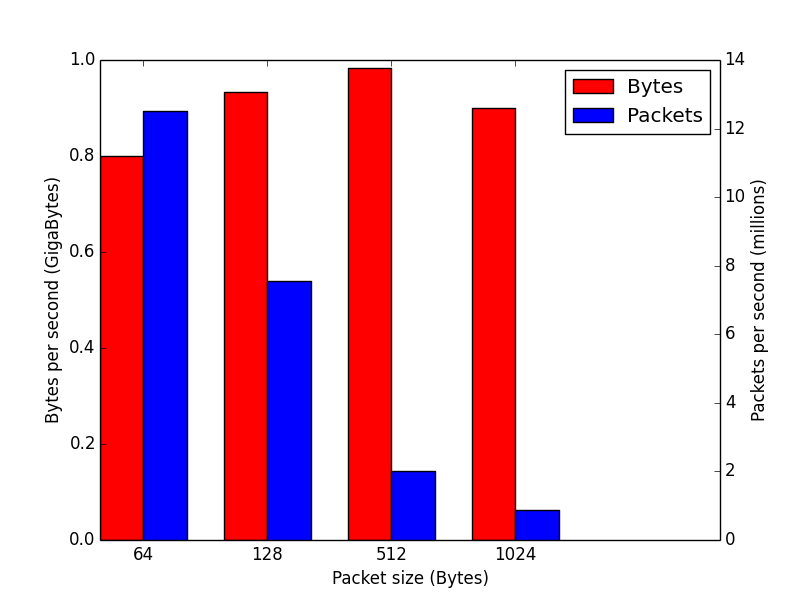
\includegraphics[width=\textwidth]{../../data/firewall/c.png}
	\caption{Firewall C implementation performance test results}
	\label{fig:firec}
\end{figure}

The results from the C implementation of the firewall are shown in \ref{fig:firec} which roughly follows the same trend from the packet capture results. The number of bytes processed per seconds roughly stays the same while the number of packets reduces as the packet size increases. Compared to the packet capture program, it has reduced byte throughput as expected due to the increased packet processing of the firewall algorithm, therefore the number of packets processed per second is slightly reduced as well.

\begin{figure}[H]
	\centering
	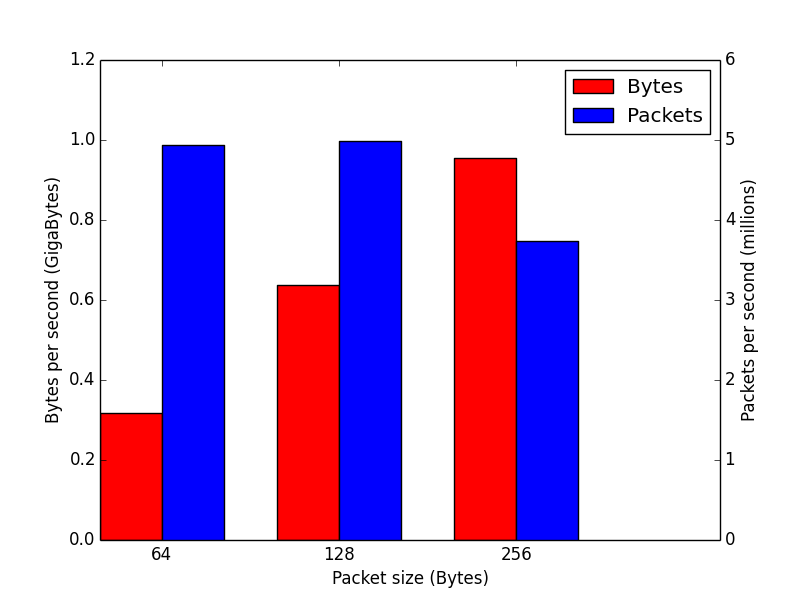
\includegraphics[width=\textwidth]{../../data/firewall/java.png}
	\caption{Firewall Java implementation performance test results}
	\label{fig:firejava}
\end{figure}

Figure \ref{fig:firejava} shows the performance of the Java implementation of a firewall. Both the packets per second and bytes per second are considerably lower than those in the C implementation. Considering the previous results for the packet capture algorithm, the only explanation for this is the extra processing per packet inspection and the transmission of packets. The packet sizes used for the performance tests were different to those used for the C test. This is because packet sizes of 512 and 1024 bytes actually stop the application from polling the packets. Instead, the NIC was dropping all of the packets as none of them were been removed from the queues. The likely cause of this is the initial configuration which all of the applications adhere to. However, this did mean that no data for packets larger than 256 bytes could be gathered for evaluation.

Using the Java profiling tool initially brought up a few minor bottlenecks which were solved before the results were taken. Afterwards, no bottlenecks could be found which were fixable and the analysis simply eluded to the inspection of the packets and the iteration over the firewall rules as the major problem.

This led to the conclusion that the only possible way to match the C performance was to increase the number of threads and receive queues per port. The idea been that performance should scale with extra threads polling packets from their own receive queues. Initial testing on this theory was carried out trying to increment the number of threads and test the performance increase. The expectation was that eventually the performance would closely relate to that of the hardware. However, problems with the application resulted in very inconsistent readings from the statistic profiler which suggested their was a problem with the affinity threads. 
Time constraints resulted in no solution to this issue and therefore no meaning full data was collected.

\subsection{Final Evaluation}
Even though the DPDKJava framework abstracts a lot of work away from the user and allows for easy programming of applications, the framework still doesn't perform to the same standard as native implementations. The performance testing on the firewall application proved this and without tests for the threaded applications no guarantee of performance matching can be made. Theoretically the performance difference can be made via adding extra threads, but extra CPU loading would then have to be taken into consideration.

This came as a real disappointment since the design consideration considered all aspects of problems within the framework and initial testing with the packet capture application looked promising.

\todo{talk about requirement to fine tune code - dont be silly}

\subsection{extrapolate for other non-native languages}
A number of other programming languages such as Visual Basic (.NET) and C\# use similar a virtual machine just like Java to make them portable to other machines. This gives the opportunity to extrapolate certain high-level implementation details and apply them to other non-native programming languages, allowing for other application not written in Java to take advantage of fast non-native packet processing. \todo{continue this, where should it go?}

\end{document}